% shortlist_loss
\begin{figure*}[t]
\centering
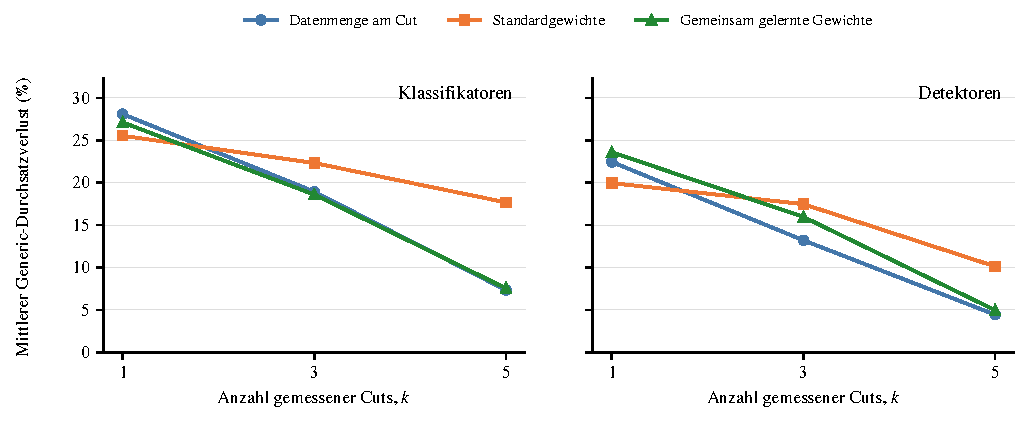
\includegraphics[width=\textwidth]{figures/shortlist_loss.pdf}
\caption{Graphbasierte Auswahl anhand des gemessenen Generic-Durchsatzes. Die Kurven zeigen den mittleren Durchsatzverlust, nachdem die ersten $k$ Cuts einer Rangfolge gemessen und der schnellste ausgewählt wurden. Klassifikatoren und Detektoren werden getrennt ausgewertet. Ein Budget von 1, 3 oder 5 bezeichnet die Zahl gemessener Cuts, nicht die Zahl zurückgehaltener Modelle. Bei weniger Kandidaten werden alle verfügbaren Cuts verwendet. Der gemeinsame Score wird auf den anderen Modellen trainiert; das Testmodell ist auf allen Beschleunigern ausgeschlossen. Dieselbe Rangfolge wird für alle drei Budgets ausgewertet. Das Trainingsziel mittelt die Verluste bei 1, 3 und 5 Cuts. Jede Gruppe erhält das gleiche Gewicht. Verfügbarer bedingter Zwischenstand: 331 qualitätszulässige Cuts in 21 Modell--Beschleuniger-Gruppen. Gemessene Qualitätsfehler (28) und offene Qualitätsentscheidungen (0) werden ausgeschlossen; bei offenen Entscheidungen bleibt die Qualitätsmenge unvollständig.}
\label{fig:rq3-shortlist-loss}
\end{figure*}

% shortlist_loss_single_column
\begin{figure}[t]
\centering
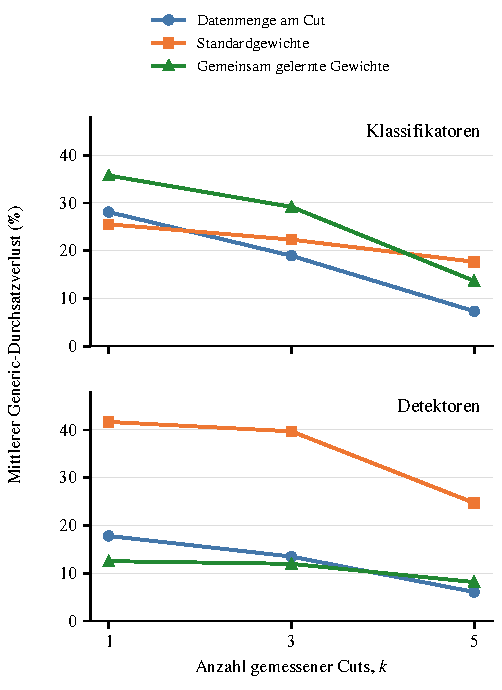
\includegraphics[width=\columnwidth]{figures/shortlist_loss_single_column.pdf}
\caption{Graphbasierte Auswahl anhand des gemessenen Generic-Durchsatzes. Die Kurven zeigen den mittleren Durchsatzverlust, nachdem die ersten $k$ Cuts einer Rangfolge gemessen und der schnellste ausgewählt wurden. Klassifikatoren und Detektoren werden getrennt ausgewertet. Ein Budget von 1, 3 oder 5 bezeichnet die Zahl gemessener Cuts, nicht die Zahl zurückgehaltener Modelle. Bei weniger Kandidaten werden alle verfügbaren Cuts verwendet. Der gemeinsame Score wird auf den anderen Modellen trainiert; das Testmodell ist auf allen Beschleunigern ausgeschlossen. Dieselbe Rangfolge wird für alle drei Budgets ausgewertet. Das Trainingsziel mittelt die Verluste bei 1, 3 und 5 Cuts. Jede Gruppe erhält das gleiche Gewicht. Verfügbarer bedingter Zwischenstand: 331 qualitätszulässige Cuts in 21 Modell--Beschleuniger-Gruppen. Gemessene Qualitätsfehler (28) und offene Qualitätsentscheidungen (0) werden ausgeschlossen; bei offenen Entscheidungen bleibt die Qualitätsmenge unvollständig.}
\label{fig:rq3-shortlist-loss-single-column}
\end{figure}

% fit_scopes_k5
\begin{figure*}[t]
\centering
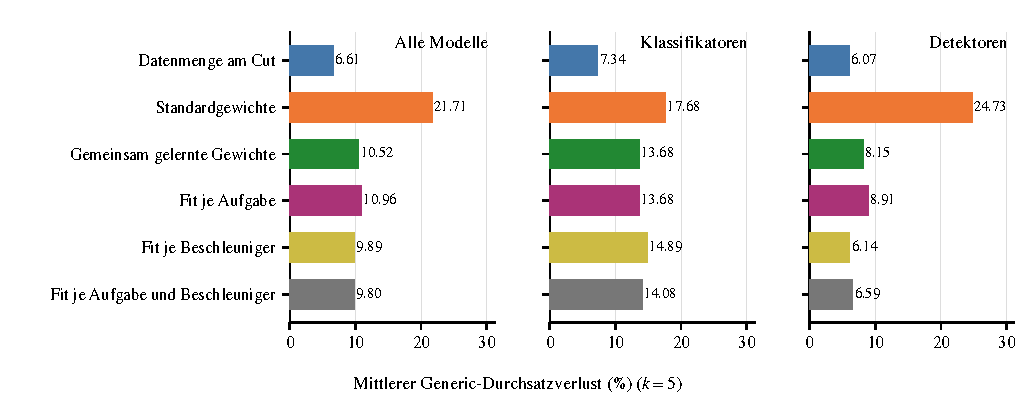
\includegraphics[width=\textwidth]{figures/fit_scopes_k5.pdf}
\caption{Mittlerer Generic-Durchsatzverlust bei einem Budget von fünf Cuts. Gemeinsame Gewichte werden mit getrennten Fits je Aufgabe, Beschleuniger und deren Kombination verglichen. In jedem Fit ist das gesamte Testmodell auf allen Beschleunigern ausgeschlossen. Das Trainingsziel mittelt die Verluste bei 1, 3 und 5 Cuts. Die Werte beschreiben den verfügbaren qualitätszulässigen Zwischenstand und sind keine neuen Native-Messungen.}
\label{fig:rq3-fit-scopes-k5}
\end{figure*}
